\chapter{Design Configuration}
\label{ch:Configuration}
This chapter elaborates on the \textit{Swing}’s configuration, using an earlier extensively performed trade-off in \Cref{sec:tradeoff} and the preliminary design of the final configuration in \Cref{sec:final_config}.


\section{Trade-Off}
\label{sec:tradeoff}
Previously, four different concepts were generated, differing in propulsion, wing and fuselage design.
These concepts are preliminary sketches in \Cref{fig:concepts4}.
A trade-off was conducted to select the best design, in which the concepts were graded based on six different criteria: transition efficiency, structural complexity, energy efficiency, safety and noise emissions.
The concepts were scored on these criteria based on preliminary calculations.

The Class I preliminary sizing and Class II sizing were conducted to perform the trade-off.
In Class I, the wing and power loading diagrams were constructed by setting constraints on the different mission phases.
An initial surface area and power were calculated using the retrieved Class I information and competitor historical data.
These values were used as input for the Class II sizing.
In the Class II sizing, a method described by \citeauthor{Ugwueze_Sizing_Method}~\cite{Ugwueze_Sizing_Method}, which relies on the Cessna II method from \citeauthor{Roskam_Part_V}~\cite{Roskam_Part_V}, was used to design the initial subsystem mass, power and geometry.
Moreover, a preliminary noise model was implemented to estimate the noise since this is a requirement set by the customers: Te-2-STK07-1-2. 
\enquote*{The noise level within the cabin shall never exceed 65 [dBA]}.
After the preliminary sizing, the trade-off was conducted, which was won by C2.1 and can be seen in \Cref{tab:performtoff}.

\begin{scriptsize} % Reduce the font size of the table
\begin{longtable}[c]{p{2.5cm}|p{1cm}|p{2cm}|p{1.3cm}|p{1.5cm}|p{1cm}|p{1.3cm}|c}
\caption{Final trade-off}
\label{tab:performtoff}\\
\diagbox[width=2.7cm]{\textbf{Concepts}}{\textbf{Criteria}}
                         & \textbf{CR-01} & \textbf{CR-02} & \textbf{CR-03} & \textbf{CR-04} & \textbf{CR-05} & \textbf{CR-06} & \textbf{Final Score}\\ \hline
\endfirsthead
%
\endhead
%
C1.5 (Winged Rotorcraft) & \cellcolor[HTML]{83C77D}Full-sized model (4) & \cellcolor[HTML]{E0E383}Excellent control, low CEF\footnote{conversion effectiveness factor} (3) & \cellcolor[HTML]{E0E383}Six moving parts, low complexity, low loads (3) & \cellcolor[HTML]{83C77D}Energy consumption 67.0 kWh (4) & \cellcolor[HTML]{63BE7B}Full redundancy (5) & \cellcolor[HTML]{E0E383}Engine noise 122.7 dB, obstruction area 9$\text{m}^2$ (3) & \cellcolor[HTML]{b2d580} \textbf{3.5}\\ \hline
C2.1 (Rotating Wing) & \cellcolor[HTML]{E0E383}Scale model highly tested (3) & \cellcolor[HTML]{63BE7B}Good control, excellent CEF (5) & \cellcolor[HTML]{E0E383}Two moving parts, low complexity, high loads (3) & \cellcolor[HTML]{E0E383}Energy consumption 73.2 kWh (3) & \cellcolor[HTML]{E0E383}Fatal hinge failure (3) & \cellcolor[HTML]{83C77D}Engine noise 125.2 dB, obstruction area 0.5$\text{m}^2$ (4) & \cellcolor[HTML]{9ace7e} \textbf{3.8} \\ \hline
C2.6 (Folding Wing) & \cellcolor[HTML]{83C77D}Full-sized model (4) & \cellcolor[HTML]{E0E383}High control, low CEF (3) & \cellcolor[HTML]{FCBF7B}Six moving parts, high complexity, medium loads (2) & \cellcolor[HTML]{83C77D}Energy consumption 66.9 kWh (4) & \cellcolor[HTML]{63BE7B}Full redundancy (5) & \cellcolor[HTML]{E0E383}Engine noise 120.6 dB, obstruction area 7.1$\text{m}^2$ (3) & \cellcolor[HTML]{c9dc82} \textbf{3.4} \\ \hline
C2.10 (Variable Skew Quad Plane) & \cellcolor[HTML]{FCBF7B}Scale model (2) & \cellcolor[HTML]{E0E383}High control, low CEF (3) & \cellcolor[HTML]{83C77D}One moving part, low complexity, medium loads (4) & \cellcolor[HTML]{FCBF7B}Energy consumption 78.4 kWh (2) & \cellcolor[HTML]{83C77D}Fail-safe (4) & \cellcolor[HTML]{FCBF7B}Engine noise 134.2 dB, obstruction area 6$\text{m}^2$ (2) & \cellcolor[HTML]{eed17f} \textbf{2.8} \\
\end{longtable}
\end{scriptsize}

\begin{figure}[H]
    \centering
    \begin{subfigure}[b]{0.35\textwidth}
        \centering
        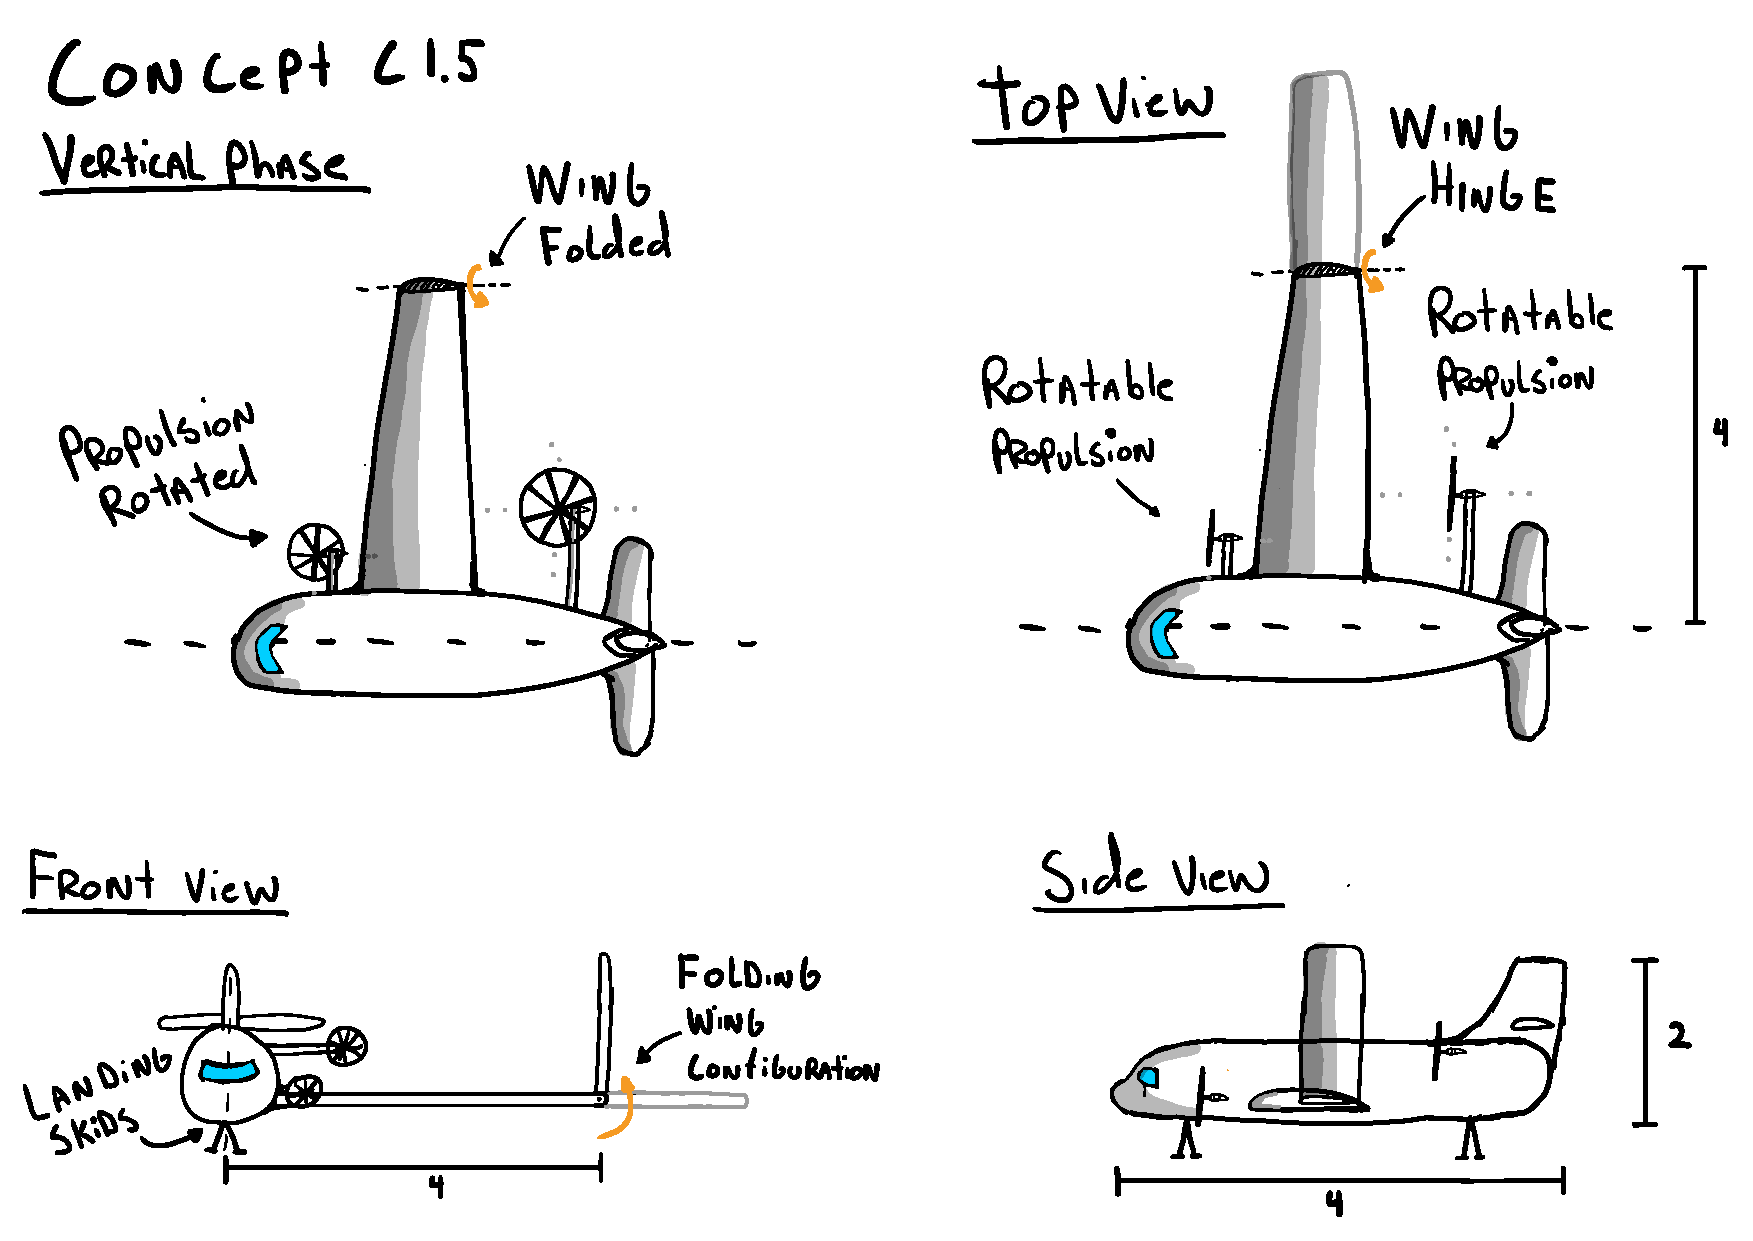
\includegraphics[width=\textwidth]{figures/Concepts/Concept C1.5 v3}
        \caption{C1.5}
        \label{fig:c15}
    \end{subfigure}
    ~
    \begin{subfigure}[b]{0.35\textwidth}
        \centering
        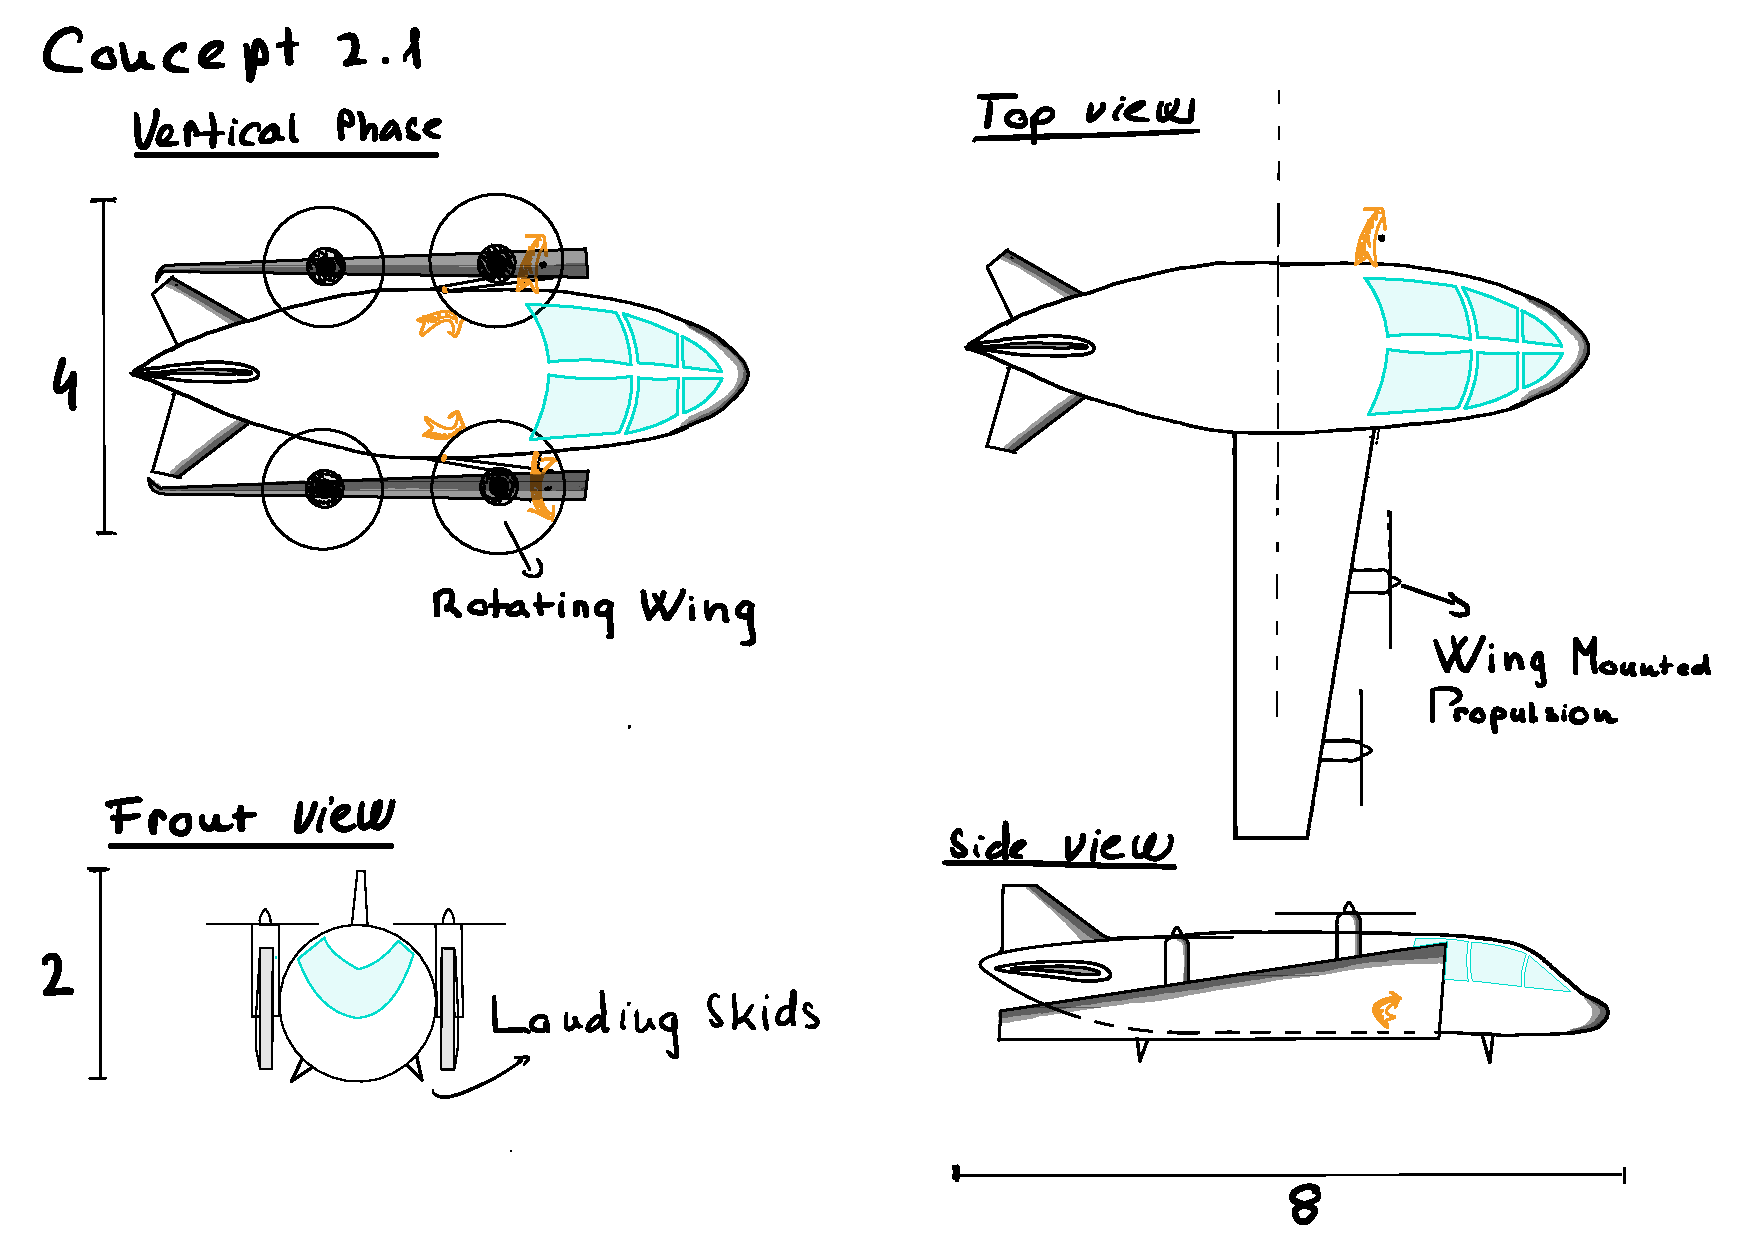
\includegraphics[width=\textwidth]{figures/Concepts/Concept C2.1 v3}
        \caption{C2.1}
        \label{fig:c21}
    \end{subfigure}
    \vskip\baselineskip % vertical space between rows
    
    \begin{subfigure}[b]{0.35\textwidth}
        \centering
        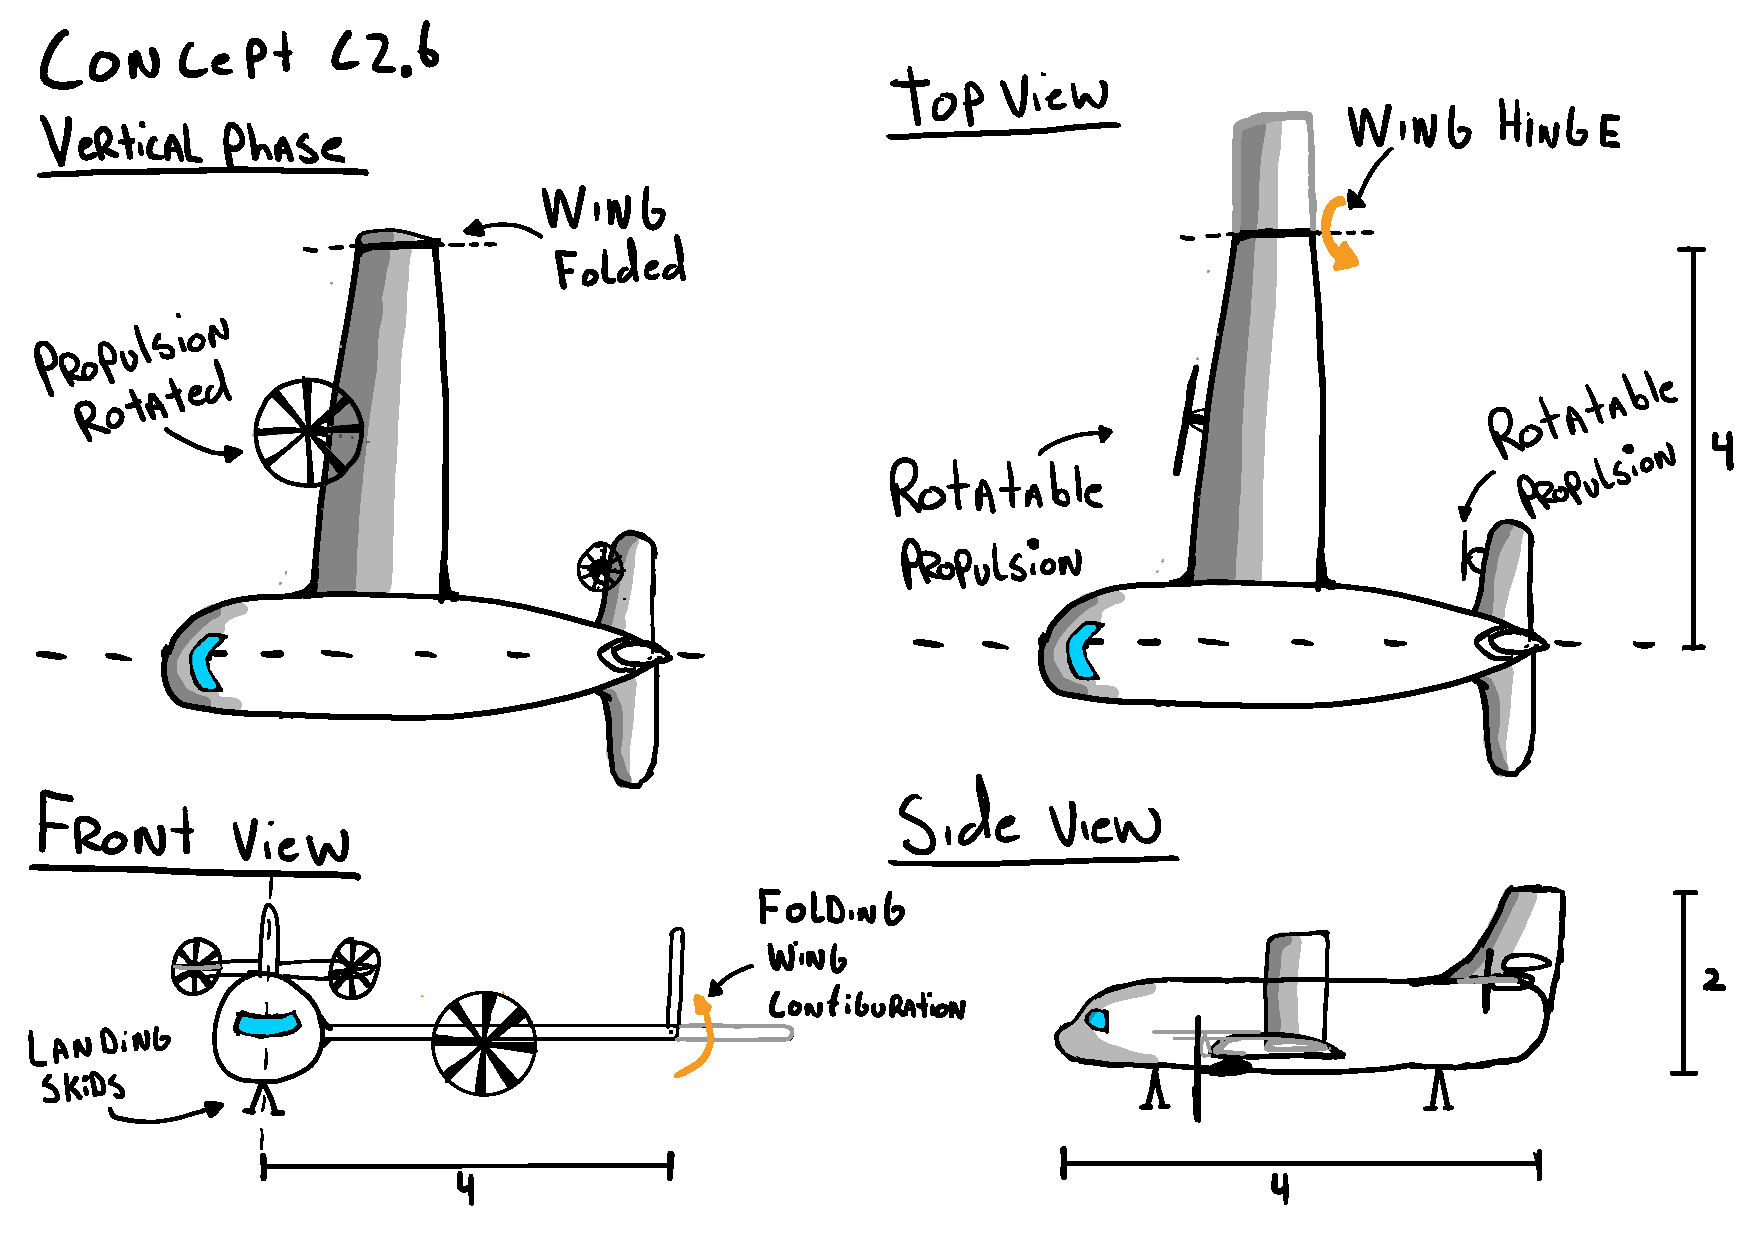
\includegraphics[width=\textwidth]{figures/Concepts/Concept C2.6 v3}
        \caption{C2.6}
        \label{fig:c26}
    \end{subfigure}
    ~
    \begin{subfigure}[b]{0.35\textwidth}
        \centering
        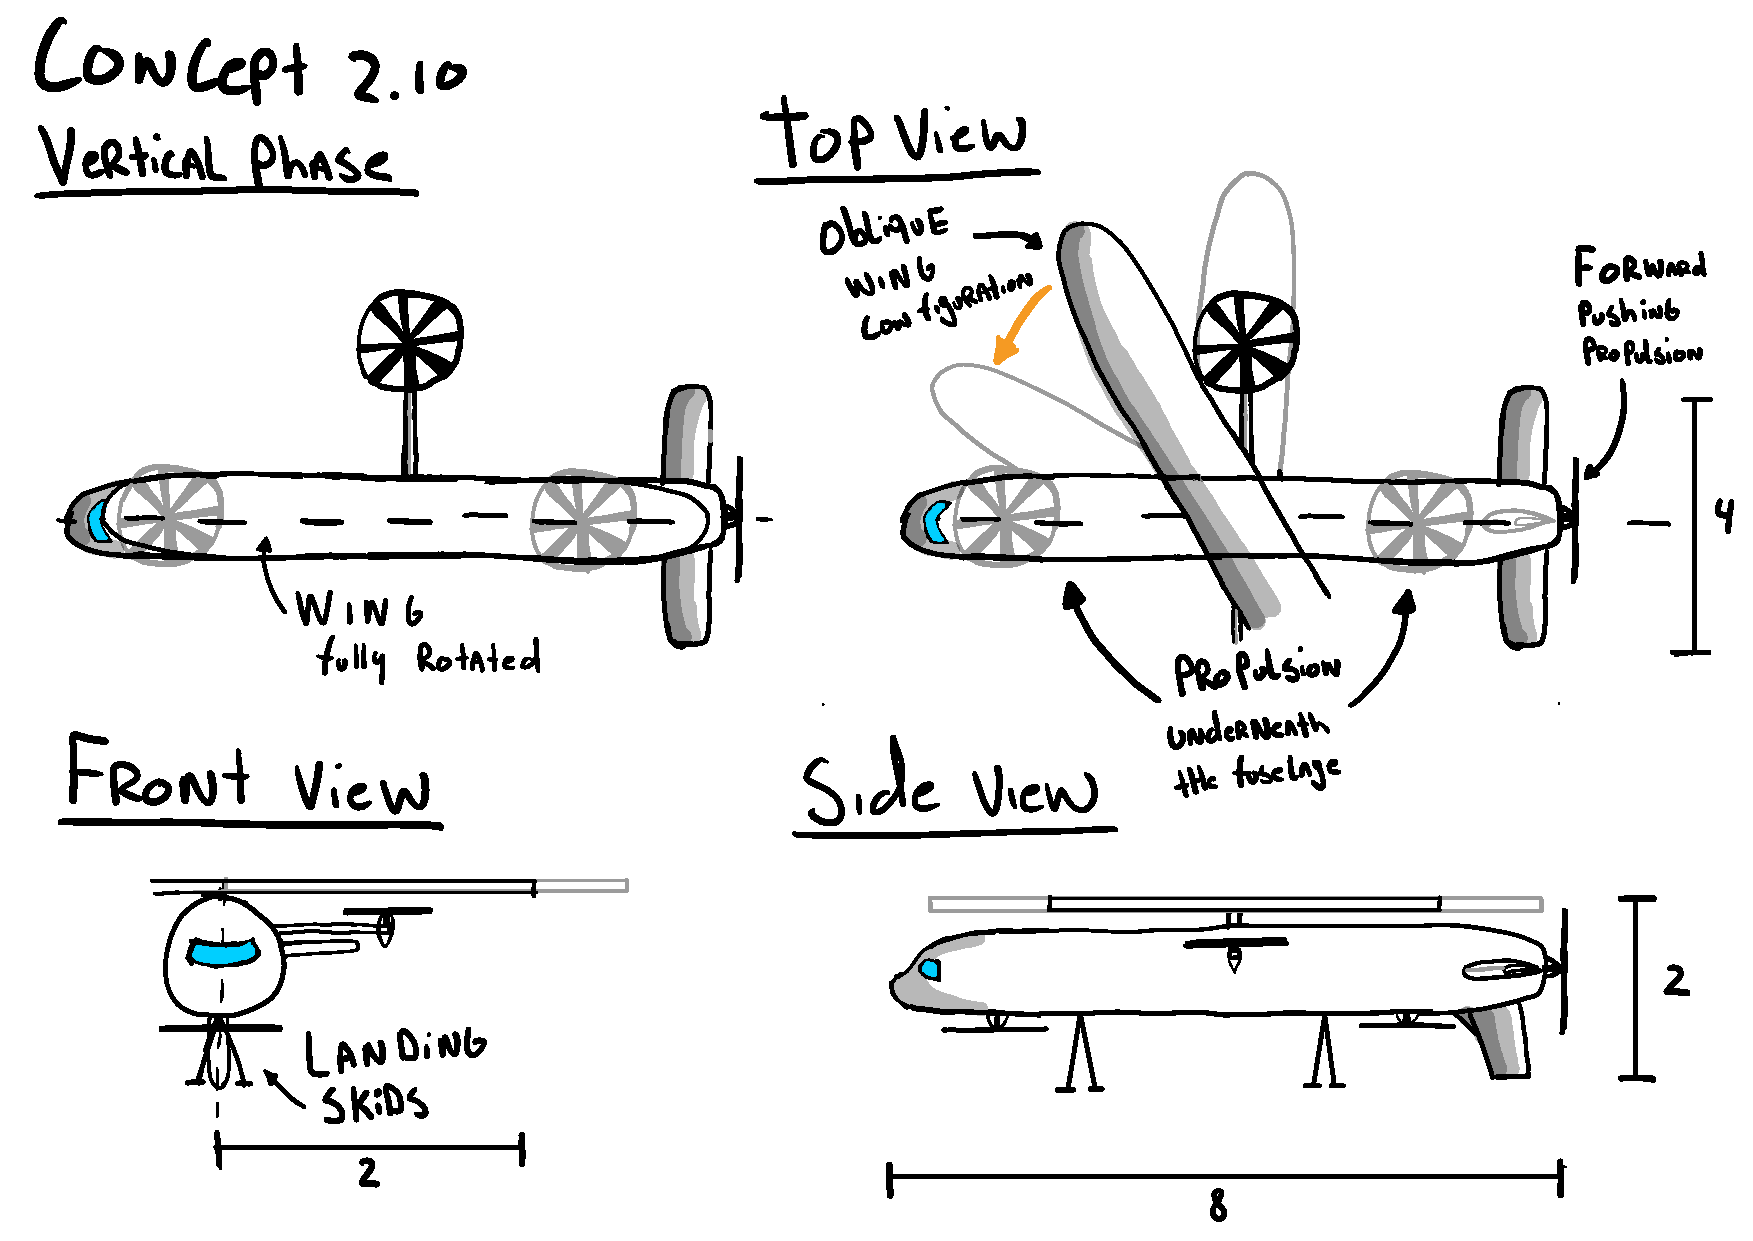
\includegraphics[width=\textwidth]{figures/Concepts/Concept C2.10 v3}
        \caption{C2.10}
        \label{fig:210}
    \end{subfigure}
    \caption{Four concepts eVTOL }
    \label{fig:concepts4}
\end{figure}

\section{Final Configuration}
\label{sec:final_config}
 The final configuration, C2.1, utilises rotating wings to take off vertically and transform into a propeller aircraft at a higher altitude, better described in \Cref{sec:mission_overview}.
 The propulsion is fixed on the wings, so it rotates with the wing from vertical to horizontal alignment.
 To do so, a special hinge with only one specific axis of rotation is designed.
 From the preliminary sizing explained above, initial design parameters were obtained, which can be seen in \Cref{tab:over_param}.
 
\begin{table}[H]
% \caption{Preliminary (left) and updated (right) parameters of the \textit{Swing eVTOL}}
\centering
\begin{minipage}{0.49\textwidth}
    \centering
    \caption{Preliminary parameters}
    \label{tab:over_param}
    \sisetup{table-format=4.1}
    \begin{tabular}{lc|S}
    \toprule
    \multicolumn{2}{c|}{\textbf{Parameter}}  & \textbf{C2.1} \\ \midrule
    Wingspan & {[}m{]}                           & 14.0           \\
    Wing surface & {[}m$^2${]}                     & 25.4       \\
    Total mass & {[}kg{]}                      & 1500  \\
    Battery mass & {[}kg{]}                     & 345    \\ \bottomrule
    \end{tabular}
\end{minipage}
~
\begin{minipage}{0.49\textwidth}
    \centering
    \caption{Updated parameters inputted}
    \label{tab:over_param_updated}
    \sisetup{table-format=4.1}
    \begin{tabular}{lc|S}
    \toprule
    \multicolumn{2}{c|}{\textbf{Parameter}}  & \textbf{C2.1} \\ \midrule
    Wingspan & {[}m{]}                           & 14.0           \\
    Wing surface & {[}m$^2${]}                     & 14.0       \\
    Total mass & {[}kg{]}                      & 1650  \\
    Battery mass & {[}kg{]}                     & 400    \\
    \bottomrule
    \end{tabular}
\end{minipage}
\end{table}


These values from \Cref{tab:over_param} have been iterated, and from these adjusted values, some critical design configuration changes have been made.
First, it was determined to use six engines instead of four because the system should be redundant and not fail if an engine fails, but also due to noise, efficiency, and downwash creation.
Moreover, a high-wing configuration was chosen because of the fuselage clearance during hover.
Subsequently, a downward V-tail was chosen because of the vertical height requirement of two meters, and it helped the landing configuration.
Finally, the wing surface area is almost halved to \qty{14}{m^2} to relieve the bending moment on the hinge and because of the overestimated lift.
All these aspects shall be discussed in more detail throughout this report.
The updated values are seen in \Cref{tab:over_param_updated}
